\documentclass{article}

% content/resources/templates/preamble.tex
\usepackage[margin=0.6in]{geometry}
\author{Milav Dabgar}
\usepackage{amsmath,amssymb,amsthm}
\usepackage{booktabs}
\usepackage{multirow}
\usepackage{xcolor}
\usepackage{tcolorbox}
\tcbuselibrary{breakable,skins}
\usepackage[colorlinks=true,linkcolor=blue]{hyperref}
\usepackage{titlesec}
\usepackage{enumitem}
\usepackage{tikz}
\usepackage{pgfplots}
\usepackage{circuitikz}
\usepackage[version=4]{mhchem}
\usepackage{longtable}
\usepackage{array}
\usepackage{float}
\usepackage{caption}
\usepackage{listings}

\lstset{
  basicstyle=\small\ttfamily,
  breaklines=true,
  breakatwhitespace=false,
  postbreak=\mbox{\textcolor{red}{$\hookrightarrow$}\space},
  float=false,
  numbers=left,
  numberstyle=\tiny\color{gray},
  numbersep=10pt,
  xleftmargin=2em,
  keywordstyle=\color{blue},
  commentstyle=\color{green!60!black},
  stringstyle=\color{purple},
  backgroundcolor=\color{gray!5},
  showstringspaces=false,
  tabsize=2,
  captionpos=b,
  keepspaces=true,
  columns=flexible
}

\pgfplotsset{compat=1.18}
\usetikzlibrary{shapes,arrows,positioning,calc,patterns,decorations.pathmorphing,decorations.markings,arrows.meta}

% Color scheme
\definecolor{headcolor}{RGB}{0,102,204}
\definecolor{keycolor}{RGB}{220,20,60}
\definecolor{solutioncolor}{RGB}{34,139,34}
\definecolor{mnemoniccolor}{RGB}{148,0,211}
\definecolor{codecolor}{RGB}{0,0,100}

% Spacing
\setlength{\parskip}{3pt}
\setlist[itemize]{nosep}
\setlist[enumerate]{nosep}

% Title formatting
\titleformat{\section}{\Large\bfseries\color{headcolor}}{\thesection}{1em}{}
\titleformat{\subsection}{\large\bfseries\color{headcolor}}{\thesubsection}{1em}{}

% Pandoc tightlist compatibility
\providecommand{\tightlist}{%
  \setlength{\itemsep}{0pt}\setlength{\parskip}{0pt}}

% Pandoc longtable compatibility
\newcounter{none}
\def\thenone{}


% content/resources/templates/english-boxes.tex

% Custom environments
\newtcolorbox{solutionbox}{
 breakable,
 enhanced,
 colback=solutioncolor!5!white,
 colframe=solutioncolor!75!black,
 fonttitle=\bfseries,
 title=Solution
}

\newtcolorbox{solutionboxnobreak}{
 colback=solutioncolor!5!white,
 colframe=solutioncolor!75!black,
 fonttitle=\bfseries,
 title=Solution
}

\newtcolorbox{keyformula}{
 breakable,
 enhanced,
 colback=keycolor!5!white,
 colframe=keycolor!75!black,
 fonttitle=\bfseries,
 title=Key Formula
}

\newtcolorbox{mnemonicboxenv}{
 breakable,
 enhanced,
 colback=mnemoniccolor!5!white,
 colframe=mnemoniccolor!75!black,
 fonttitle=\bfseries,
 title=Mnemonic
}

\newcommand{\mnemonicbox}[1]{%
  \begin{mnemonicboxenv}
    #1
  \end{mnemonicboxenv}
}


% Custom commands for GTU solutions
% This file defines semantic commands for consistent formatting

% Question command with automatic formatting
\newcommand{\question}[2]{%
  \section*{Question #1}%
  \textbf{#2}%
}

% OR question variant
\newcommand{\questionor}[2]{%
  \section*{Question #1 OR}%
  \textbf{#2}%
}

% Proper table environment with caption
\newenvironment{answertable}[1]{%
  \begin{table}[htbp]
  \centering
  \caption{#1}
}{%
  \end{table}
}

% Proper figure environment for diagrams
\newenvironment{answerdiagram}[1]{%
  \begin{figure}[htbp]
  \centering
  \caption{#1}
}{%
  \end{figure}
}

% Semantic markup for key terms
\newcommand{\keyword}[1]{\textbf{#1}}
\newcommand{\code}[1]{\texttt{#1}}
\newcommand{\classname}[1]{\texttt{#1}}
\newcommand{\methodname}[1]{\texttt{#1}}

% Proper quotation marks
\newcommand{\mnemonic}[1]{``#1''}


\title{Linux Operating System (4331602) - Summer 2024 Solution}
\date{June 10, 2024}

\begin{document}
\maketitle

\questionmarks{1(a)}{3}{Define Operating System and give its goal.}

\begin{solutionbox}
\textbf{Operating System Definition}: A program that acts as an interface between computer hardware and users, managing system resources and controlling program execution.

\textbf{Goals of Operating System}:

\begin{center}
\captionof{table}{OS Goals}
\begin{tabulary}{\linewidth}{|L|L|}
\hline
\textbf{Goal} & \textbf{Description} \\ \hline
\keyword{Resource Management} & Efficiently allocate CPU, memory, I/O devices \\ \hline
\keyword{User Convenience} & Provide easy-to-use interface \\ \hline
\keyword{System Protection} & Secure system from unauthorized access \\ \hline
\end{tabulary}
\end{center}
\end{solutionbox}

\begin{mnemonicbox}
\mnemonic{RUS: Resource management, User convenience, System protection}
\end{mnemonicbox}

\questionmarks{1(b)}{4}{Give name Components of Computer System \& Explain need of Operating system.}

\begin{solutionbox}
\textbf{Computer System Components}:

\begin{center}
\begin{tikzpicture}[node distance=1.5cm, auto]
    \node [gtu block] (users) {Users};
    \node [gtu block, below=of users] (apps) {Application Programs};
    \node [gtu block, below=of apps] (os) {Operating System};
    \node [gtu block, below=of os] (hardware) {Hardware (CPU, Memory, I/O)};
    
    \path [gtu arrow] (users) -- (apps);
    \path [gtu arrow] (apps) -- (os);
    \path [gtu arrow] (os) -- (hardware);
    \path [gtu arrow] (hardware) -- (os);
    \path [gtu arrow] (os) -- (apps);
    \path [gtu arrow] (apps) -- (users);
\end{tikzpicture}
\captionof{figure}{Computer System Hierarchy}
\end{center}

\textbf{Need of Operating System}:

\begin{itemize}
    \item \keyword{Resource Manager}: Controls hardware allocation
    \item \keyword{Interface Provider}: Easy communication between user and hardware
    \item \keyword{Security}: Protects system from threats
    \item \keyword{Error Handling}: Manages system errors efficiently
\end{itemize}
\end{solutionbox}

\begin{mnemonicbox}
\mnemonic{RISE: Resource management, Interface, Security, Error handling}
\end{mnemonicbox}

\questionmarks{1(c)}{7}{Explain below types of Operating system.}

\begin{solutionbox}
\textbf{I. Batch Operating System}

\begin{center}
\captionof{table}{Batch OS}
\begin{tabulary}{\linewidth}{|L|L|}
\hline
\textbf{Feature} & \textbf{Description} \\ \hline
\keyword{Processing} & Jobs processed in batches without user interaction \\ \hline
\keyword{Efficiency} & High throughput, low user interaction \\ \hline
\keyword{Example} & IBM mainframes \\ \hline
\end{tabulary}
\end{center}

\textbf{II. Multiprogramming Operating System}

\begin{center}
\captionof{table}{Multiprogramming OS}
\begin{tabulary}{\linewidth}{|L|L|}
\hline
\textbf{Feature} & \textbf{Description} \\ \hline
\keyword{Concept} & Multiple programs in memory simultaneously \\ \hline
\keyword{CPU Usage} & Better CPU utilization \\ \hline
\keyword{Advantage} & Reduced idle time \\ \hline
\end{tabulary}
\end{center}

\textbf{III. Time Sharing Operating System}

\begin{center}
\captionof{table}{Time Sharing OS}
\begin{tabulary}{\linewidth}{|L|L|}
\hline
\textbf{Feature} & \textbf{Description} \\ \hline
\keyword{Time Slices} & CPU time divided among users \\ \hline
\keyword{Response} & Quick response time \\ \hline
\keyword{Example} & Unix, Linux \\ \hline
\end{tabulary}
\end{center}
\end{solutionbox}

\begin{mnemonicbox}
\mnemonic{BMT: Batch, Multiprogramming, Time-sharing}
\end{mnemonicbox}

\questionmarks{1(c) OR}{7}{Explain Linux Architecture \& characteristics with its components.}

\begin{solutionbox}
\textbf{Linux Architecture}:

\begin{center}
\begin{tikzpicture}[node distance=1.2cm]
    \node [rectangle, draw, fill=blue!10, text width=8cm, text centered, minimum height=1cm] (users) {User Applications / Compilers};
    \node [rectangle, draw, fill=green!10, text width=8cm, text centered, minimum height=1cm, below=0.5cm of users] (shell) {Shell / System Libraries};
    \node [rectangle, draw, fill=red!10, text width=8cm, text centered, minimum height=1.5cm, below=0.5cm of shell] (kernel) {Linux Kernel\\(File System, Memory Mgmt, Process Mgmt, Device Drivers)};
    \node [rectangle, draw, fill=gray!20, text width=8cm, text centered, minimum height=1cm, below=0.5cm of kernel] (hardware) {Hardware (CPU, RAM, I/O Device)};
    
    \path [gtu arrow] (users) -- (shell);
    \path [gtu arrow] (shell) -- (kernel);
    \path [gtu arrow] (kernel) -- (hardware);
\end{tikzpicture}
\captionof{figure}{Linux Architecture}
\end{center}

\textbf{Linux Characteristics}:

\begin{center}
\captionof{table}{Characteristics}
\begin{tabulary}{\linewidth}{|L|L|}
\hline
\textbf{Characteristic} & \textbf{Description} \\ \hline
\keyword{Open Source} & Free and modifiable \\ \hline
\keyword{Multiuser} & Multiple users simultaneously \\ \hline
\keyword{Multitasking} & Multiple processes concurrently \\ \hline
\keyword{Portable} & Runs on various hardware \\ \hline
\end{tabulary}
\end{center}

\textbf{Components}:
\begin{itemize}
    \item \keyword{Kernel}: Core of operating system
    \item \keyword{Shell}: Command interpreter
    \item \keyword{File System}: Organizes data storage
\end{itemize}
\end{solutionbox}

\begin{mnemonicbox}
\mnemonic{COMP: Core, Open source, Multiuser, Portable}
\end{mnemonicbox}

\questionmarks{2(a)}{3}{Describe Process Control Block. And define (1) PID (2) stack pointer (3) program counter}

\begin{solutionbox}
\textbf{Process Control Block (PCB)}: Data structure containing process information for OS management.

\textbf{Definitions}:

\begin{center}
\captionof{table}{PCB Definitions}
\begin{tabulary}{\linewidth}{|L|L|}
\hline
\textbf{Term} & \textbf{Definition} \\ \hline
\keyword{PID} & Process Identifier - unique number for each process \\ \hline
\keyword{Stack Pointer} & Points to top of process stack \\ \hline
\keyword{Program Counter} & Contains address of next instruction \\ \hline
\end{tabulary}
\end{center}
\end{solutionbox}

\begin{mnemonicbox}
\mnemonic{PSP: PID, Stack pointer, Program counter}
\end{mnemonicbox}

\questionmarks{2(b)}{4}{Describe the Process Model and Process states}

\begin{solutionbox}
\textbf{Process Model}: Conceptual representation of how processes are managed by OS.

\textbf{Process States}:

\begin{center}
\begin{tikzpicture}[node distance=2cm, auto]
    \node [gtu state] (new) {New};
    \node [gtu state, right=of new] (ready) {Ready};
    \node [gtu state, right=of ready] (running) {Running};
    \node [gtu state, right=of running] (terminated) {Terminated};
    \node [gtu state, below=of ready] (waiting) {Waiting};
    
    \path [gtu arrow] (new) -- (ready);
    \path [gtu arrow] (ready) -- node[yshift=0.2cm] {Dispatch} (running);
    \path [gtu arrow] (running) -- node[above] {Exit} (terminated);
    \path [gtu arrow] (running) -- node[right] {I/O Wait} (waiting);
    \path [gtu arrow] (waiting) -- node[left] {I/O Complete} (ready);
    \path [gtu arrow] (running) edge[bend right=45] node[above] {Interrupt} (ready);
\end{tikzpicture}
\captionof{figure}{Process State Diagram}
\end{center}

\begin{center}
\captionof{table}{Process States}
\begin{tabulary}{\linewidth}{|L|L|}
\hline
\textbf{State} & \textbf{Description} \\ \hline
\keyword{New} & Process being created \\ \hline
\keyword{Ready} & Waiting for CPU \\ \hline
\keyword{Running} & Executing instructions \\ \hline
\keyword{Waiting} & Waiting for I/O \\ \hline
\keyword{Terminated} & Process finished \\ \hline
\end{tabulary}
\end{center}
\end{solutionbox}

\begin{mnemonicbox}
\mnemonic{NRRWT: New, Ready, Running, Waiting, Terminated}
\end{mnemonicbox}

\questionmarks{2(c)}{7}{Demonstrate Scheduling Algorithm:(I) First Come First Serve, (II) Shortest Job First}

\begin{solutionbox}
\textbf{I. First Come First Serve (FCFS)}

\begin{center}
\captionof{table}{FCFS Scheduling}
\begin{tabulary}{\linewidth}{|C|C|C|C|C|}
\hline
\textbf{Process} & \textbf{Arrival} & \textbf{Burst} & \textbf{Completion} & \textbf{Turnaround} \\ \hline
P1 & 0 & 4 & 4 & 4 \\ \hline
P2 & 1 & 3 & 7 & 6 \\ \hline
P3 & 2 & 2 & 9 & 7 \\ \hline
\end{tabulary}
\end{center}

\textbf{Average Turnaround Time} = (4+6+7)/3 = 5.67

\textbf{II. Shortest Job First (SJF)}

\begin{center}
\captionof{table}{SJF Scheduling}
\begin{tabulary}{\linewidth}{|C|C|C|C|C|}
\hline
\textbf{Process} & \textbf{Arrival} & \textbf{Burst} & \textbf{Completion} & \textbf{Turnaround} \\ \hline
P3 & 2 & 2 & 4 & 2 \\ \hline
P2 & 1 & 3 & 7 & 6 \\ \hline
P1 & 0 & 4 & 11 & 11 \\ \hline
\end{tabulary}
\end{center}

\textbf{Average Turnaround Time} = (2+6+11)/3 = 6.33
\end{solutionbox}

\begin{mnemonicbox}
\mnemonic{FS: FCFS (First order), SJF (Shortest first)}
\end{mnemonicbox}

\questionmarks{2(a) OR}{3}{Define Race condition, Mutual Exclusion}

\begin{solutionbox}
\begin{center}
\captionof{table}{Race vs Mutual Exclusion}
\begin{tabulary}{\linewidth}{|L|L|}
\hline
\textbf{Term} & \textbf{Definition} \\ \hline
\keyword{Race Condition} & Multiple processes access shared data simultaneously causing inconsistent results \\ \hline
\keyword{Mutual Exclusion} & Only one process can access critical section at a time \\ \hline
\end{tabulary}
\end{center}

\textbf{Example}: Two processes updating same bank account balance.
\end{solutionbox}

\begin{mnemonicbox}
\mnemonic{RM: Race (simultaneous access), Mutual (one at a time)}
\end{mnemonicbox}

\questionmarks{2(b) OR}{4}{Define all Throughput, Turnaround Time, Waiting Time, Response Time}

\begin{solutionbox}
\begin{center}
\captionof{table}{Scheduling Metrics}
\begin{tabulary}{\linewidth}{|L|L|}
\hline
\textbf{Term} & \textbf{Definition} \\ \hline
\keyword{Throughput} & Number of processes completed per unit time \\ \hline
\keyword{Turnaround Time} & Total time from submission to completion \\ \hline
\keyword{Waiting Time} & Time spent waiting in ready queue \\ \hline
\keyword{Response Time} & Time from submission to first response \\ \hline
\end{tabulary}
\end{center}

\textbf{Formulae}:
\begin{itemize}
    \item \textbf{Turnaround Time} = Completion Time - Arrival Time
    \item \textbf{Waiting Time} = Turnaround Time - Burst Time
    \item \textbf{Response Time} = First CPU Time - Arrival Time
\end{itemize}
\end{solutionbox}

\begin{mnemonicbox}
\mnemonic{TTWR: Throughput, Turnaround, Waiting, Response}
\end{mnemonicbox}

\questionmarks{2(c) OR}{7}{Explain Round Robin Algorithm with example.}

\begin{solutionbox}
\textbf{Round Robin}: Each process gets equal CPU time slice (quantum).

\textbf{Example} (Time Quantum = 2):

\begin{center}
\captionof{table}{RR Example Processes}
\begin{tabulary}{\linewidth}{|C|C|}
\hline
\textbf{Process} & \textbf{Burst Time} \\ \hline
P1 & 5 \\ \hline
P2 & 3 \\ \hline
P3 & 4 \\ \hline
\end{tabulary}
\end{center}

\textbf{Execution Timeline}:

\begin{center}
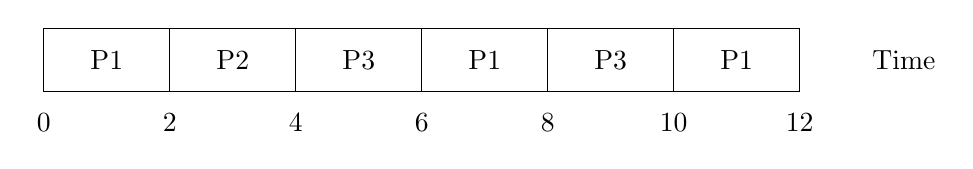
\begin{tikzpicture}[x=0.8cm, y=0.8cm]
    \draw (0,0) rectangle (2,1) node[midway] {P1};
    \draw (2,0) rectangle (4,1) node[midway] {P2};
    \draw (4,0) rectangle (6,1) node[midway] {P3};
    \draw (6,0) rectangle (8,1) node[midway] {P1};
    \draw (8,0) rectangle (10,1) node[midway] {P3};
    \draw (10,0) rectangle (12,1) node[midway] {P1};
    
    \foreach \x in {0,2,4,6,8,10,12}
        \node at (\x, -0.5) {\x};
        
    \node [anchor=west] at (13,0.5) {Time};
\end{tikzpicture}
\captionof{figure}{RR Execution Timeline}
\end{center}

\begin{center}
\captionof{table}{RR Results}
\begin{tabulary}{\linewidth}{|C|C|C|}
\hline
\textbf{Process} & \textbf{Completion Time} & \textbf{Turnaround Time} \\ \hline
P1 & 12 & 12 \\ \hline
P2 & 6 & 6 \\ \hline
P3 & 10 & 10 \\ \hline
\end{tabulary}
\end{center}

\textbf{Average Turnaround Time} = (12+6+10)/3 = 9.33

\textbf{Advantages}:
\begin{itemize}
    \item \keyword{Fair}: Equal time to all processes
    \item \keyword{Responsive}: Good for interactive systems
\end{itemize}
\end{solutionbox}

\begin{mnemonicbox}
\mnemonic{RR-FE: Round Robin gives Fair and Equal time}
\end{mnemonicbox}

\questionmarks{3(a)}{3}{Give File Access Methods type}

\begin{solutionbox}
\begin{center}
\captionof{table}{File Access Methods}
\begin{tabulary}{\linewidth}{|L|L|}
\hline
\textbf{Method} & \textbf{Description} \\ \hline
\keyword{Sequential} & Read/write in order from beginning \\ \hline
\keyword{Direct} & Access any record directly \\ \hline
\keyword{Indexed} & Use index to locate records \\ \hline
\end{tabulary}
\end{center}
\end{solutionbox}

\begin{mnemonicbox}
\mnemonic{SDI: Sequential, Direct, Indexed}
\end{mnemonicbox}

\questionmarks{3(b)}{4}{Give Deadlock characteristics and Describe: Deadlock Prevention, Deadlock Avoidance}

\begin{solutionbox}
\textbf{Deadlock Characteristics}:

\begin{center}
\captionof{table}{Deadlock Conditions}
\begin{tabulary}{\linewidth}{|L|L|}
\hline
\textbf{Condition} & \textbf{Description} \\ \hline
\keyword{Mutual Exclusion} & Resources cannot be shared \\ \hline
\keyword{Hold and Wait} & Process holds resource while waiting \\ \hline
\keyword{No Preemption} & Resources cannot be forcibly taken \\ \hline
\keyword{Circular Wait} & Circular chain of waiting processes \\ \hline
\end{tabulary}
\end{center}

\textbf{Deadlock Prevention}: Remove any one of four conditions.

\textbf{Deadlock Avoidance}: Use algorithms like Banker's algorithm to avoid unsafe states.
\end{solutionbox}

\begin{mnemonicbox}
\mnemonic{MHNC: Mutual exclusion, Hold and wait, No preemption, Circular wait}
\end{mnemonicbox}

\questionmarks{3(c)}{7}{Explain the File Allocation Methods Contiguous, linked, indexed}

\begin{solutionbox}
\textbf{File Allocation Methods}:

\begin{center}
\captionof{table}{Allocation Methods Comparison}
\begin{tabulary}{\linewidth}{|L|L|L|L|}
\hline
\textbf{Method} & \textbf{Description} & \textbf{Advantage} & \textbf{Disadvantage} \\ \hline
\keyword{Contiguous} & Sequential blocks & Fast access & External fragmentation \\ \hline
\keyword{Linked} & Scattered blocks with pointers & No fragmentation & Slow random access \\ \hline
\keyword{Indexed} & Index block contains addresses & Fast random access & Extra overhead \\ \hline
\end{tabulary}
\end{center}

\textbf{I. Contiguous Allocation}:

\begin{center}
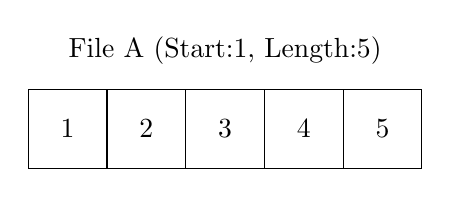
\begin{tikzpicture}[node distance=0cm, outer sep=0pt]
    \node [rectangle, draw, minimum width=1cm, minimum height=1cm] (b1) {1};
    \node [rectangle, draw, minimum width=1cm, minimum height=1cm, right=of b1] (b2) {2};
    \node [rectangle, draw, minimum width=1cm, minimum height=1cm, right=of b2] (b3) {3};
    \node [rectangle, draw, minimum width=1cm, minimum height=1cm, right=of b3] (b4) {4};
    \node [rectangle, draw, minimum width=1cm, minimum height=1cm, right=of b4] (b5) {5};
    \node [above=0.2cm of b3] {File A (Start:1, Length:5)};
\end{tikzpicture}
\captionof{figure}{Contiguous Allocation}
\end{center}

\textbf{II. Linked Allocation}:

\begin{center}
\begin{tikzpicture}[node distance=1cm, auto]
    \node [gtu state] (b1) {1};
    \node [gtu state, right=of b1] (b7) {7};
    \node [gtu state, right=of b7] (b3) {3};
    \node [gtu state, right=of b3] (b9) {9};
    \node [gtu state, right=of b9] (null) {NULL};
    
    \path [gtu arrow] (b1) -- (b7);
    \path [gtu arrow] (b7) -- (b3);
    \path [gtu arrow] (b3) -- (b9);
    \path [gtu arrow] (b9) -- (null);
\end{tikzpicture}
\captionof{figure}{Linked Allocation}
\end{center}

\textbf{III. Indexed Allocation}:

\begin{center}
\begin{tikzpicture}[node distance=1.5cm]
    \node [rectangle, draw, fill=yellow!10, inner sep=0pt] (index) {\begin{tabular}{c}Index Block\\ \hline 1\\3\\7\\9\\12\end{tabular}};
    \node [gtu block, right=of index, yshift=1.5cm] (b1) {Block 1};
    \node [gtu block, right=of index, yshift=0.7cm] (b3) {Block 3};
    \node [gtu block, right=of index, yshift=-0.1cm] (b7) {Block 7};
    \node [gtu block, right=of index, yshift=-1.5cm] (b9) {Block 9};
    
    \draw [->] (index.east) -- (b1.west);
    \draw [->] (index.east) -- (b3.west);
    \draw [->] (index.east) -- (b7.west);
    \draw [->] (index.east) -- (b9.west);
\end{tikzpicture}
\captionof{figure}{Indexed Allocation}
\end{center}
\end{solutionbox}

\begin{mnemonicbox}
\mnemonic{CLI: Contiguous, Linked, Indexed}
\end{mnemonicbox}

\questionmarks{3(a) OR}{3}{Give knowledge Linux File System Structure}

\begin{solutionbox}
\textbf{Linux File System Hierarchy}:

\begin{center}
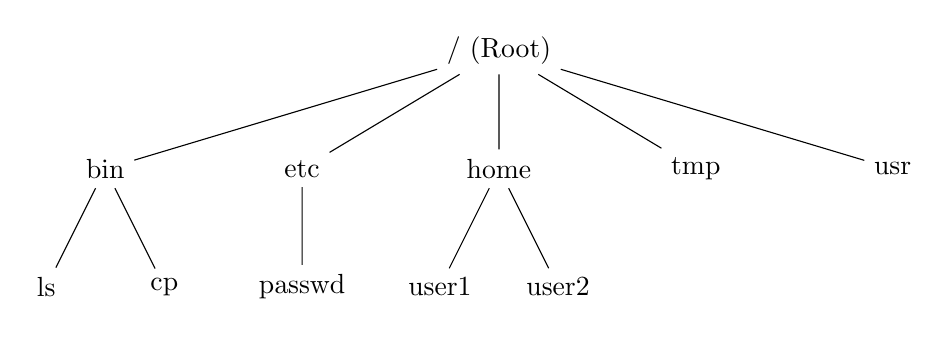
\begin{tikzpicture}[level distance=1.5cm, level 1/.style={sibling distance=2.5cm}, level 2/.style={sibling distance=1.5cm}]
    \node {/ (Root)}
        child {node {bin}
            child {node {ls}}
            child {node {cp}}
        }
        child {node {etc}
            child {node {passwd}}
        }
        child {node {home}
            child {node {user1}}
            child {node {user2}}
        }
        child {node {tmp}}
        child {node {usr}};
\end{tikzpicture}
\captionof{figure}{File System Tree}
\end{center}

\begin{center}
\captionof{table}{Key Directories}
\begin{tabulary}{\linewidth}{|L|L|}
\hline
\textbf{Directory} & \textbf{Purpose} \\ \hline
\keyword{/bin} & Essential system binaries \\ \hline
\keyword{/etc} & System configuration files \\ \hline
\keyword{/home} & User home directories \\ \hline
\end{tabulary}
\end{center}
\end{solutionbox}

\begin{mnemonicbox}
\mnemonic{BEH: Bin, Etc, Home}
\end{mnemonicbox}

\questionmarks{3(b) OR}{4}{Explain Critical Section and Semaphore with example.}

\begin{solutionbox}
\textbf{Critical Section}: Code segment accessing shared resources.

\textbf{Critical Section Structure}:
\begin{itemize}
    \item \keyword{Entry}: Request permission
    \item \keyword{Critical}: Access shared resource
    \item \keyword{Exit}: Release permission
    \item \keyword{Remainder}: Other code
\end{itemize}

\textbf{Semaphore}: Synchronization tool using counter variable.

\textbf{Example}:
\begin{lstlisting}[language=bash,caption={Binary Semaphore}]
# Binary Semaphore Operations
wait(S):
  while S <= 0 do nothing
  S = S - 1

signal(S):
  S = S + 1
\end{lstlisting}
\end{solutionbox}

\begin{mnemonicbox}
\mnemonic{ECER: Entry, Critical, Exit, Remainder}
\end{mnemonicbox}

\questionmarks{3(c) OR}{7}{Define and explain Deadlock Avoidance, Deadlock Detection and Recovery}

\begin{solutionbox}
\textbf{Deadlock Avoidance}:
\begin{itemize}
    \item Uses \keyword{Banker's Algorithm}
    \item Checks if resource allocation leads to safe state
\end{itemize}

\textbf{Deadlock Detection}:
\begin{itemize}
    \item Periodically checks for deadlock using \keyword{Wait-for Graph}
\end{itemize}

\begin{center}
\begin{tikzpicture}[node distance=2cm, auto]
    \node [circle, draw] (p1) {P1};
    \node [circle, draw, right=of p1] (p2) {P2};
    \node [circle, draw, below=of p2] (p3) {P3};
    
    \path [gtu arrow] (p1) -- (p2);
    \path [gtu arrow] (p2) -- (p3);
    \path [gtu arrow] (p3) edge[bend left] (p1);
\end{tikzpicture}
\captionof{figure}{Wait-for Graph (Detection)}
\end{center}

\textbf{Deadlock Recovery Methods}:

\begin{center}
\captionof{table}{Recovery Methods}
\begin{tabulary}{\linewidth}{|L|L|}
\hline
\textbf{Method} & \textbf{Description} \\ \hline
\keyword{Process Termination} & Kill deadlocked processes \\ \hline
\keyword{Resource Preemption} & Take resources from processes \\ \hline
\keyword{Rollback} & Return to previous safe state \\ \hline
\end{tabulary}
\end{center}
\end{solutionbox}

\begin{mnemonicbox}
\mnemonic{ADR: Avoidance, Detection, Recovery}
\end{mnemonicbox}

\questionmarks{4(a)}{3}{Why Need of file Protection explain?}

\begin{solutionbox}
\textbf{Need for File Protection}:

\begin{center}
\captionof{table}{Protection Needs}
\begin{tabulary}{\linewidth}{|L|L|}
\hline
\textbf{Reason} & \textbf{Description} \\ \hline
\keyword{Privacy} & Protect personal data \\ \hline
\keyword{Security} & Prevent unauthorized access \\ \hline
\keyword{Integrity} & Maintain data consistency \\ \hline
\end{tabulary}
\end{center}

\textbf{Protection Mechanisms}:
\begin{itemize}
    \item Access Control Lists (ACL)
    \item File Permissions (Read, Write, Execute)
    \item User Authentication
\end{itemize}
\end{solutionbox}

\begin{mnemonicbox}
\mnemonic{PSI: Privacy, Security, Integrity}
\end{mnemonicbox}

\questionmarks{4(b)}{4}{Illustrate Program threats, System threats}

\begin{solutionbox}
\textbf{Program Threats}:
\begin{itemize}
    \item \keyword{Virus}: Self-replicating malicious code
    \item \keyword{Worm}: Network-spreading malware
    \item \keyword{Trojan Horse}: Disguised malicious program
\end{itemize}

\textbf{System Threats}:
\begin{itemize}
    \item \keyword{Denial of Service}: Overwhelm system resources
    \item \keyword{Port Scanning}: Find vulnerable services
    \item \keyword{Man-in-Middle}: Intercept communications
\end{itemize}
\end{solutionbox}

\begin{mnemonicbox}
\mnemonic{VWT-DPM: Virus, Worm, Trojan; DoS, Port scan, Man-in-middle}
\end{mnemonicbox}

\questionmarks{4(c)}{7}{Briefly detailing Operating System security policies and procedures}

\begin{solutionbox}
\textbf{Security Policies}:

\begin{center}
\captionof{table}{Security Policies}
\begin{tabulary}{\linewidth}{|L|L|}
\hline
\textbf{Policy} & \textbf{Description} \\ \hline
\keyword{Access Control} & Who can access what resources \\ \hline
\keyword{Authentication} & Verify user identity \\ \hline
\keyword{Authorization} & Determine user permissions \\ \hline
\keyword{Audit} & Monitor and log activities \\ \hline
\end{tabulary}
\end{center}

\textbf{Security Procedures Flow}:

\begin{center}
\begin{tikzpicture}[node distance=1.5cm, auto]
    \node [gtu state] (login) {User Login};
    \node [gtu decision, right=of login] (auth) {Auth?};
    \node [gtu state, right=of auth] (access) {Access};
    \node [gtu state, below=of access] (log) {Log Activity};
    \node [gtu state, below=of login] (deny) {Deny};
    
    \path [gtu arrow] (login) -- (auth);
    \path [gtu arrow] (auth) -- node[above] {Yes} (access);
    \path [gtu arrow] (auth) -- node[left] {No} (deny);
    \path [gtu arrow] (access) -- (log);
\end{tikzpicture}
\captionof{figure}{Security Flow}
\end{center}

\textbf{Implementation Steps}:
\begin{enumerate}
    \item User Registration and credential setup
    \item Multi-factor Authentication
    \item Role-based Access Control
    \item Regular Security Audits
\end{enumerate}
\end{solutionbox}

\begin{mnemonicbox}
\mnemonic{AAAA: Access control, Authentication, Authorization, Audit}
\end{mnemonicbox}

\questionmarks{4(a) OR}{3}{Give idea Authentication and Authorization.}

\begin{solutionbox}
\begin{center}
\captionof{table}{Auth vs Authz}
\begin{tabulary}{\linewidth}{|L|L|L|}
\hline
\textbf{Term} & \textbf{Definition} & \textbf{Example} \\ \hline
\keyword{Authentication} & Verify user identity & Username/password \\ \hline
\keyword{Authorization} & Determine access rights & File permissions \\ \hline
\end{tabulary}
\end{center}

\textbf{Authentication Methods}:
\begin{itemize}
    \item Password-based
    \item Biometric
    \item Token-based
\end{itemize}
\end{solutionbox}

\begin{mnemonicbox}
\mnemonic{AA: Authentication (who), Authorization (what)}
\end{mnemonicbox}

\questionmarks{4(b) OR}{4}{Explain Operating System security policies and procedures}

\begin{solutionbox}
\textbf{Security Policies Framework}:

\begin{center}
\captionof{table}{Security Framework}
\begin{tabulary}{\linewidth}{|L|L|}
\hline
\textbf{Component} & \textbf{Purpose} \\ \hline
\keyword{User Management} & Control user accounts \\ \hline
\keyword{Data Protection} & Secure sensitive information \\ \hline
\keyword{Network Security} & Protect communications \\ \hline
\keyword{System Monitoring} & Detect threats \\ \hline
\end{tabulary}
\end{center}
\end{solutionbox}

\begin{mnemonicbox}
\mnemonic{UDNS: User, Data, Network, System}
\end{mnemonicbox}

\questionmarks{4(c) OR}{7}{Detailing the Security measures in Operating System}

\begin{solutionbox}
\textbf{Comprehensive Security Measures}:
\begin{itemize}
    \item \keyword{Physical}: Server room access, bio locks
    \item \keyword{Network}: Firewalls, VPN
    \item \keyword{System}: Antivirus, patches
    \item \keyword{Application}: Secure coding
    \item \keyword{Data}: Encryption, backups
\end{itemize}

\textbf{Access Control Matrix Example}:
\begin{center}
\captionof{table}{Access Matrix}
\begin{tabulary}{\linewidth}{|L|C|C|}
\hline
\textbf{User} & \textbf{File A} & \textbf{File B} \\ \hline
Admin & RWX & RWX \\ \hline
User1 & RW- & R-- \\ \hline
Guest & R-- & --- \\ \hline
\end{tabulary}
\end{center}

\textbf{Security Implementation Timeline}:

\begin{center}
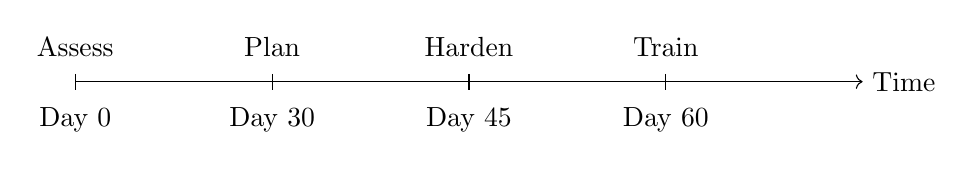
\begin{tikzpicture}
    \draw [->] (0,0) -- (10,0) node[right] {Time};
    
    \foreach \x in {0,2.5,5,7.5}
        \draw (\x, 0.1) -- (\x, -0.1);
        
    \node [anchor=north] at (0,-0.2) {Day 0};
    \node [anchor=south] at (0,0.2) {Assess};
    
    \node [anchor=north] at (2.5,-0.2) {Day 30};
    \node [anchor=south] at (2.5,0.2) {Plan};
    
    \node [anchor=north] at (5,-0.2) {Day 45};
    \node [anchor=south] at (5,0.2) {Harden};
    
    \node [anchor=north] at (7.5,-0.2) {Day 60};
    \node [anchor=south] at (7.5,0.2) {Train};
\end{tikzpicture}
\captionof{figure}{Implementation Timeline}
\end{center}
\end{solutionbox}

\begin{mnemonicbox}
\mnemonic{PNSAD: Physical, Network, System, Application, Data}
\end{mnemonicbox}

\questionmarks{5(a)}{3}{Give five Basic commands: calendar, date}

\begin{solutionbox}
\textbf{Basic Linux Commands}:

\begin{center}
\captionof{table}{Basic Commands}
\begin{tabulary}{\linewidth}{|L|L|L|}
\hline
\textbf{Command} & \textbf{Function} & \textbf{Example} \\ \hline
\code{cal} & Display calendar & \code{cal 2024} \\ \hline
\code{date} & Show current date/time & \code{date +\%d/\%m/\%Y} \\ \hline
\code{who} & Show logged users & \code{who} \\ \hline
\code{pwd} & Print working directory & \code{pwd} \\ \hline
\code{clear} & Clear screen & \code{clear} \\ \hline
\end{tabulary}
\end{center}
\end{solutionbox}

\begin{mnemonicbox}
\mnemonic{CDWPC: Cal, Date, Who, Pwd, Clear}
\end{mnemonicbox}

\questionmarks{5(b)}{4}{Explain Linux File and Directory Commands: ls, cat, mkdir, rmdir, pwd.}

\begin{solutionbox}
\textbf{File and Directory Commands}:

\begin{center}
\captionof{table}{File Commands}
\begin{tabulary}{\linewidth}{|L|L|L|}
\hline
\textbf{Command} & \textbf{Function} & \textbf{Example} \\ \hline
\code{ls} & List directory contents & \code{ls -la} \\ \hline
\code{cat} & Display file content & \code{cat file.txt} \\ \hline
\code{mkdir} & Create directory & \code{mkdir newdir} \\ \hline
\code{rmdir} & Remove empty directory & \code{rmdir olddir} \\ \hline
\end{tabulary}
\end{center}

\textbf{Usage Examples}:
\begin{lstlisting}[language=bash,caption={File Commands}]
# List files with details
ls -l /home/user

# Create multiple directories
mkdir -p dir1/dir2/dir3

# Display file with line numbers
cat -n document.txt
\end{lstlisting}
\end{solutionbox}

\begin{mnemonicbox}
\mnemonic{LCMRP: List, Cat, Mkdir, Rmdir, Pwd}
\end{mnemonicbox}

\questionmarks{5(c)}{7}{Understand and apply control statements Write a shell script to perform given operations: Write a shell script to find maximum number among three numbers.}

\begin{solutionbox}
\begin{lstlisting}[language=bash,caption={Maximum of 3 Numbers}]
#!/bin/bash
# Script to find maximum of three numbers

echo "Enter three numbers:"
read -p "First number: " num1
read -p "Second number: " num2
read -p "Third number: " num3

# Method 1: Using if-elif-else
if [ $num1 -ge $num2 ] && [ $num1 -ge $num3 ]; then
    max=$num1
elif [ $num2 -ge $num1 ] && [ $num2 -ge $num3 ]; then
    max=$num2
else
    max=$num3
fi

echo "Maximum number is: $max"
\end{lstlisting}

\textbf{Comparison Operators}:
\begin{itemize}
    \item \code{-gt}: Greater than
    \item \code{-ge}: Greater than or equal to
    \item \code{-eq}: Equal to
\end{itemize}
\end{solutionbox}

\begin{mnemonicbox}
\mnemonic{IER: If (condition), Echo (output), Read (input)}
\end{mnemonicbox}

\questionmarks{5(a) OR}{3}{What is Linux Process commands: top, ps, kill}

\begin{solutionbox}
\textbf{Linux Process Commands}:

\begin{center}
\captionof{table}{Process Commands}
\begin{tabulary}{\linewidth}{|L|L|L|}
\hline
\textbf{Command} & \textbf{Function} & \textbf{Usage} \\ \hline
\code{top} & Display running processes & \code{top} \\ \hline
\code{ps} & Show process status & \code{ps aux} \\ \hline
\code{kill} & Terminate process & \code{kill PID} \\ \hline
\end{tabulary}
\end{center}

\textbf{Details}:
\begin{itemize}
    \item \code{top}: Real-time CPU/Memory usage
    \item \code{ps -aux}: Full detailed process list
    \item \code{kill -9 PID}: Force kill a process
\end{itemize}
\end{solutionbox}

\begin{mnemonicbox}
\mnemonic{TPK: Top, Ps, Kill}
\end{mnemonicbox}

\questionmarks{5(b) OR}{4}{Linux File and Directory Commands: rm, mv,split,diff, grep}

\begin{solutionbox}
\textbf{Advanced File Commands}:

\begin{center}
\captionof{table}{Advanced Commands}
\begin{tabulary}{\linewidth}{|L|L|L|}
\hline
\textbf{Cmd} & \textbf{Function} & \textbf{Example} \\ \hline
\code{rm} & Remove files & \code{rm -rf folder} \\ \hline
\code{mv} & Move/rename & \code{mv old new} \\ \hline
\code{split} & Split files & \code{split -l 50 f.txt} \\ \hline
\code{diff} & Compare files & \code{diff f1 f2} \\ \hline
\code{grep} & Search text & \code{grep "err" log} \\ \hline
\end{tabulary}
\end{center}
\end{solutionbox}

\begin{mnemonicbox}
\mnemonic{RMSDG: Remove, Move, Split, Diff, Grep}
\end{mnemonicbox}

\questionmarks{5(c) OR}{7}{Write a shell script to read five numbers from user and find average of five numbers.}

\begin{solutionbox}
\begin{lstlisting}[language=bash,caption={Average of 5 Numbers}]
#!/bin/bash
# Script to calculate average of five numbers

echo "=== Average Calculator ==="
sum=0

echo "Enter 5 numbers:"
for i in {1..5}; do
    read -p "Enter number $i: " num
    sum=$((sum + num))
done

# Calculate average
average=$((sum / 5))

echo "--------------------------------"
echo "Sum: $sum"
echo "Average: $average"
echo "--------------------------------"
\end{lstlisting}

\textbf{Key Concepts}:
\begin{itemize}
    \item \code{\$(())}: Arithmetic expansion
    \item \code{for}: Loop for iteration
    \item \code{read}: User input
\end{itemize}
\end{solutionbox}

\begin{mnemonicbox}
\mnemonic{RSAR: Read, Sum, Average, Result}
\end{mnemonicbox}

\end{document}

